\chapter{Funktionalität}

\section{Programmfunktionalitäten}
\subsection{Funktionsübersicht}

\textbf{/F101/}\\[-0.2cm]

\textbf{/F102/}\\[-0.2cm]

\textbf{/F103/}\\[-0.2cm]

\textbf{/F201/} Jedes Neuronale Netz kann mit dem Gradienten-Abstieg-Algorithmus trainiert werden. Dabei sind die Trainingsparameter \emph{Lernrate}, \emph{Stapelgröße}, \emph{Anzahl der Trainingsbilder} und \emph{Zyklenanzahl} frei wählbar. Das Training kann manuell gestartet und gestoppt werden.\\[-0.2cm]

\textbf{/F202/} Der Nutzer soll über eine Ausgabe-Konsole über den Trainingsstand und die Genauigkeit des Neuronalen Netzes informiert werden.

\textbf{/F203/} Ein trainiertes Neuronales Netz kann bei Bedarf gespeichert oder verworfen werden werden. Wird das trainierte Netz, z.B. durch die Auswahl eines anderen Neuronalen Netzes, verworfen, ist dies auf der Konsole auszugeben. \\[-0.2cm]

\textbf{/F301/} Die Metadaten (Name, Beschreibung) eines Neuronalen Netzes sollen konfigurierbar sein.\\[-0.2cm]

\textbf{/F302/} Die Topologie des Netzes sowie die Eigenschaften von Knoten und Knotenverbindungen sollen über eine Json-Struktur bearbeitbar sein.\footnote{Es wird keine Validierung des eingegebenen Json-Strings vorgenommen. Im Rahmen des Projektes wird davon Ausgegangen, dass der Administrator weiß, welche Netztopologien zulässig sind -- z.B. eine Eingabeschicht mit $48 \times 48$ Eingabeknoten und eine Ausgabeschicht mit 10 Ausgabeknoten.}\\[-0.2cm]

\textbf{/F303/} Die in /F301/ und /F302/ am Neuronalen Netz vorgenommenen Änderungen sollen gespeichert werden können.\\[-0.2cm]

\textbf{/F304/} Es ist möglich ein neues Neuronales Netz anzulegen.\\[-0.2cm]


\subsection{Arbeitsflüsse}

\textbf{Aktivitätsdiagramm aus Anwendersicht.}

\textbf{Aktivitätsdiagramm aus Administrationssicht.} Der Administrationsbereich der Anwendung setzt sich aus zwei Unterseiten zusammen, nämlich einer Seite für die Konfiguration der Trainingsparameter (vgl. Abb. \ref{xxx}) sowie für die Bearbeitung der Neuronalen Netze (vgl. Abb. \ref{yyy}). Der Arbeitsfluss zwischen beiden Seiten ist im folgenden Aktivitätsdiagramm dargestellt.

\begin{figure}[H]
\begin{center}
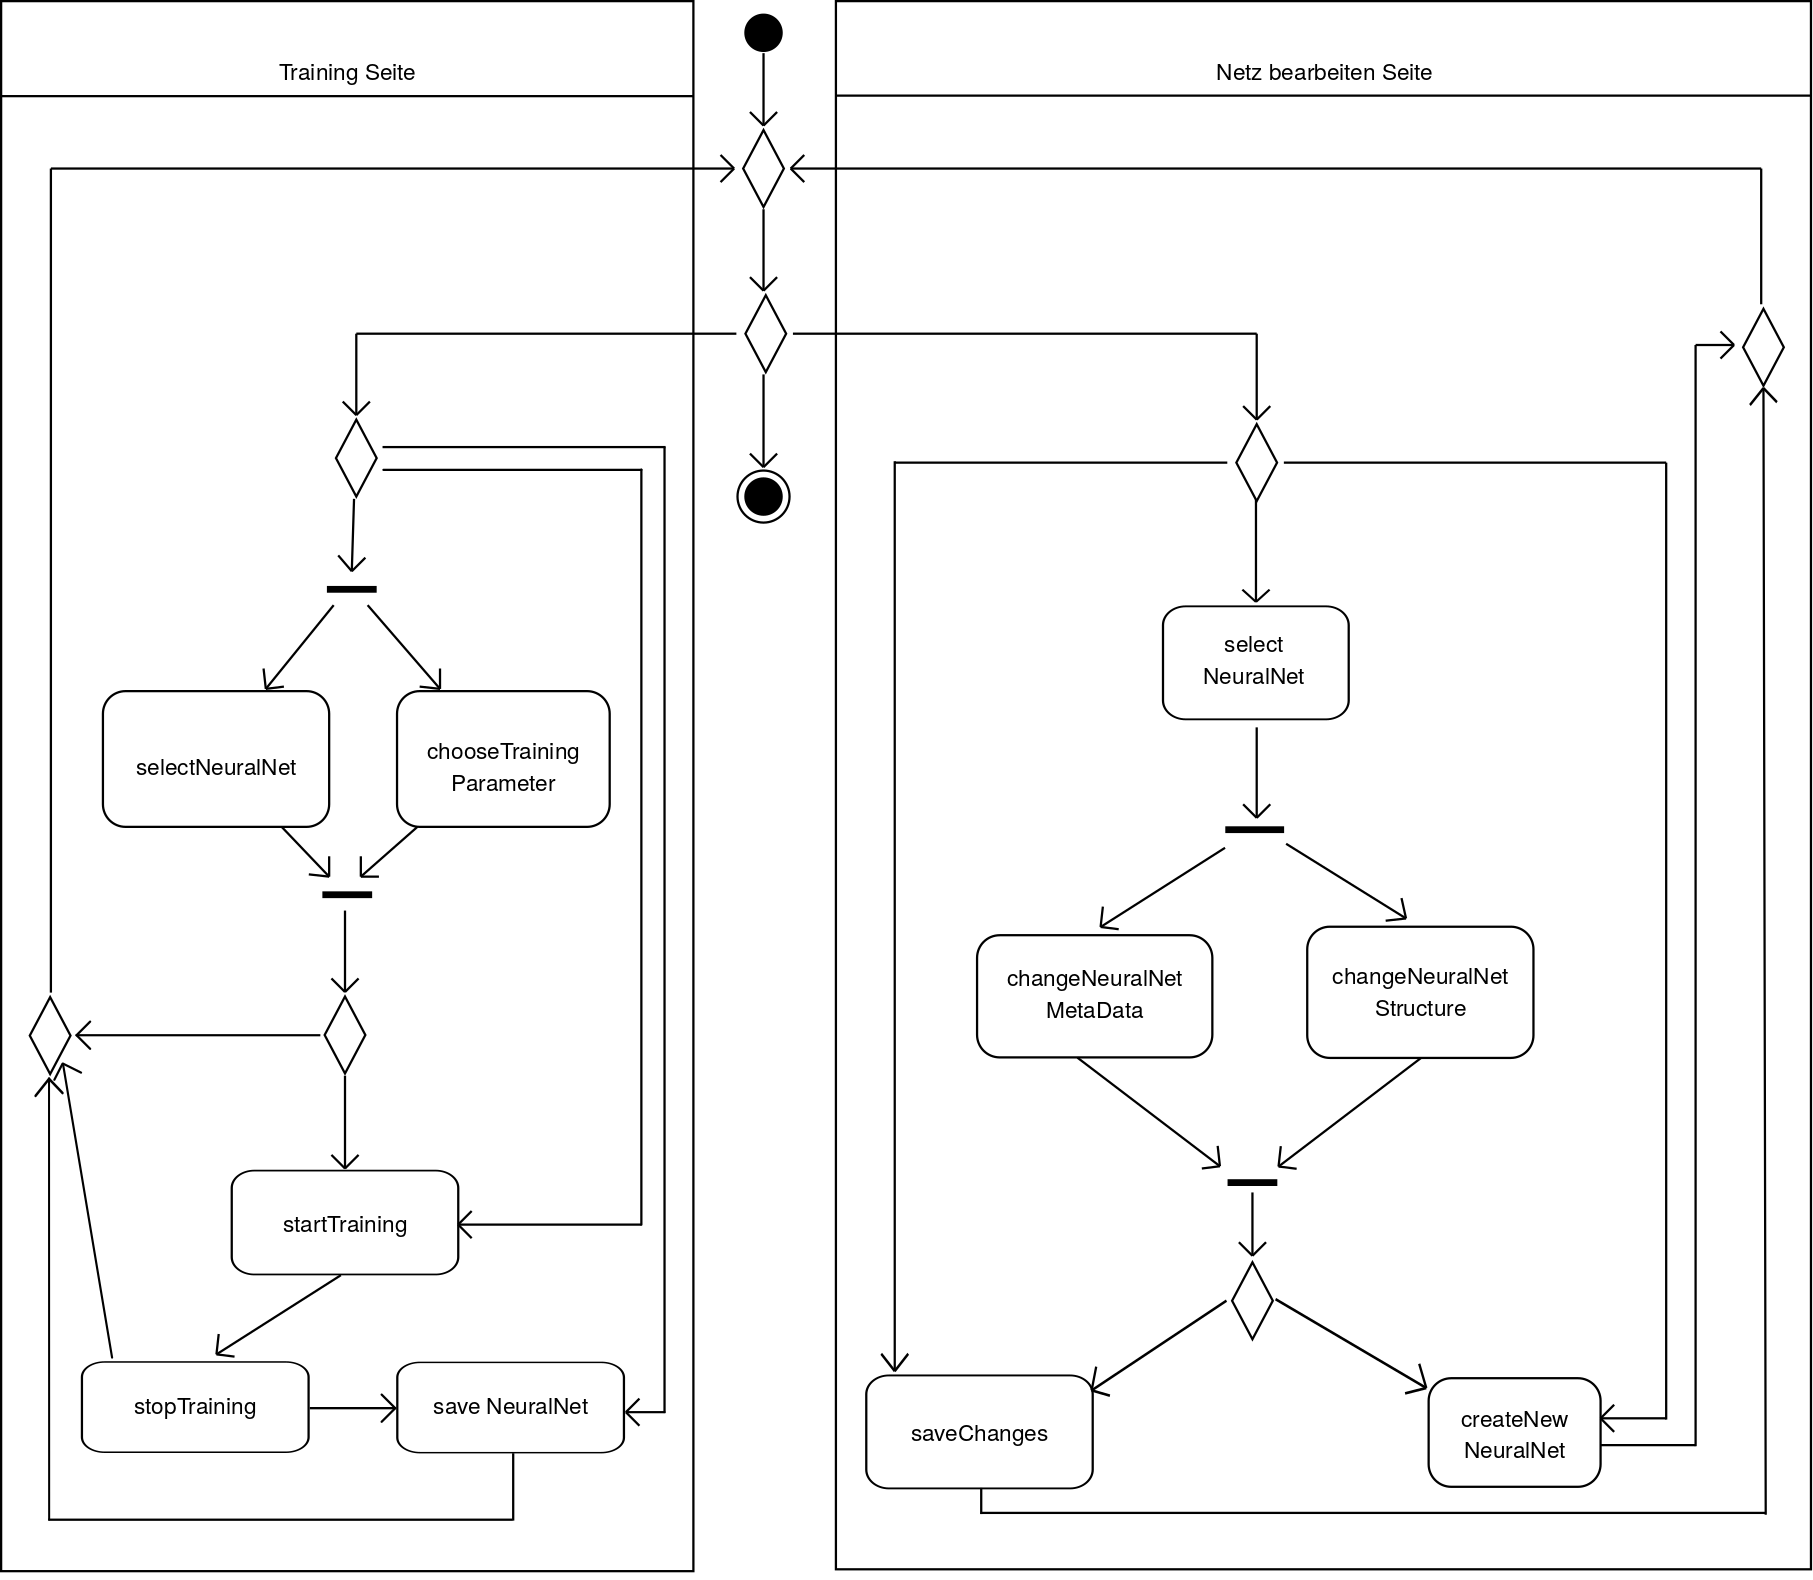
\includegraphics[width=\textwidth]{Abbildungen/UML/jan/trainingConfigAD.png}
\caption{Aktivitätsdiagramm für die Verwendung des Programmes im Administrationsbereich.}
\label{fig_trainingConfigAD}
\end{center}
\end{figure}

\section{Globale Programmarchitektur}

Zur Entkopplung einzelner Module und leichteren Wartbarkeit verwendet die Anwendung eine Drei-Schichten Architektur bestehend ausXX	 Nutzeroberfläche, Business-Schicht und Daten-Schicht. 
\begin{figure}[H]
\begin{center}
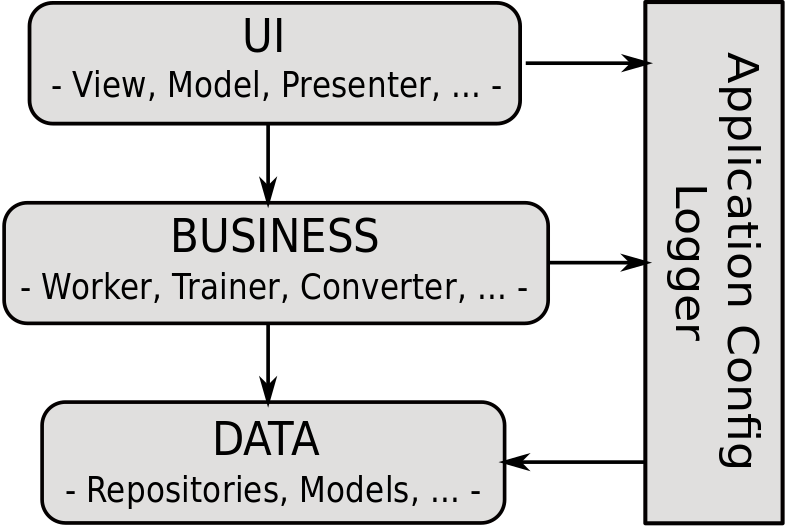
\includegraphics[width=10cm]{Abbildungen/UML/jan/SchichtenModell.png}
\end{center}
\end{figure}
Die Nutzeroberfläche dient der Nutzerinteraktion sowie der Darstellung der Eingabe- sowie verarbeiteten Daten. Sie implementiert dabei das MVP-Muster...

\textcolor{red}{ @Daniel: Hier bitte dein Part für das MVP-Pattern rein!!!}


In der Buisiness-Schicht werden alle fachspezifischen Verarbeitungen vorgenommen. Hierunter fallen beispielsweise die Vorwärtsberechnung sowie das Training eines künstlichen neuronalen Netzes oder die Konvertierung von Daten. Dazu werden für jede Entität spezifizsche Worker-Klassen bereitgestellt, die diese Aufgaben durchführen können.

\begin{figure}[H]
\begin{center}
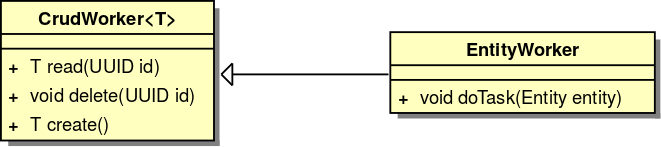
\includegraphics[width=10cm]{Abbildungen/UML/jan/workerClassDiagramm.png}
\end{center}
\end{figure}

Als unterste Schicht der Anwendung dient die Daten-Schicht der Persistierung von Daten. Hierfür stehen ihr diverse, von CRUD-Workern angesprochene Repositories zur Verfügung, die je nach Bedarf Daten (hier im Wesentlichen das Neuronale Netz) in eine Datenbank oder externe Dateien schreiben können.

In den nächsten Unterabschnitten folgt die ausführliche Beschreibung und geplante Umsetzung der von der Anwendung zu erbringenden Funktionalitäten.  

\section{Sequenz- und Klassendiagramme}
\subsection{Anwendersicht}

\textbf{/F101/}

\begin{figure}[h]
\begin{center}
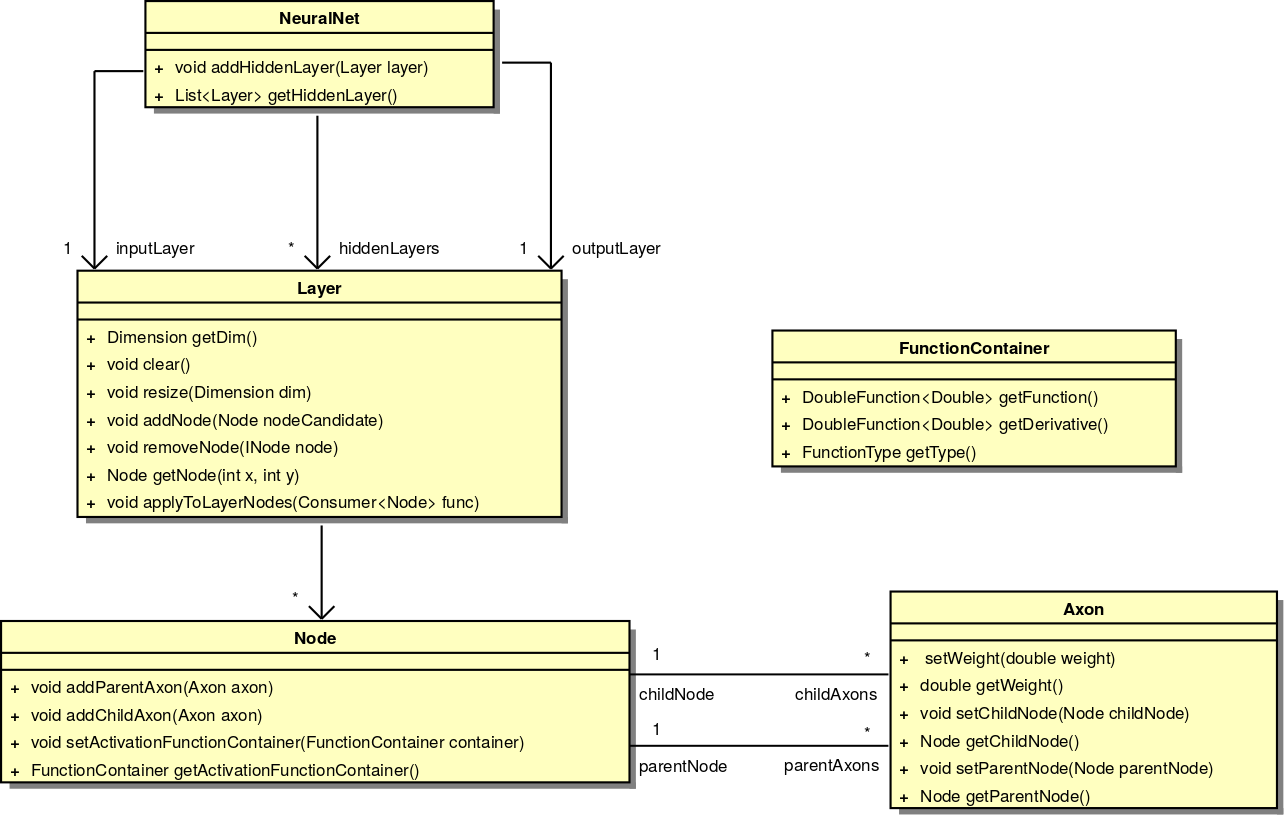
\includegraphics[width=\textwidth]{Abbildungen/UML/uml_ronny/neuralNetKlassenDiagramm.png}
\end{center}
\end{figure}


\begin{figure}[H]
\begin{center}
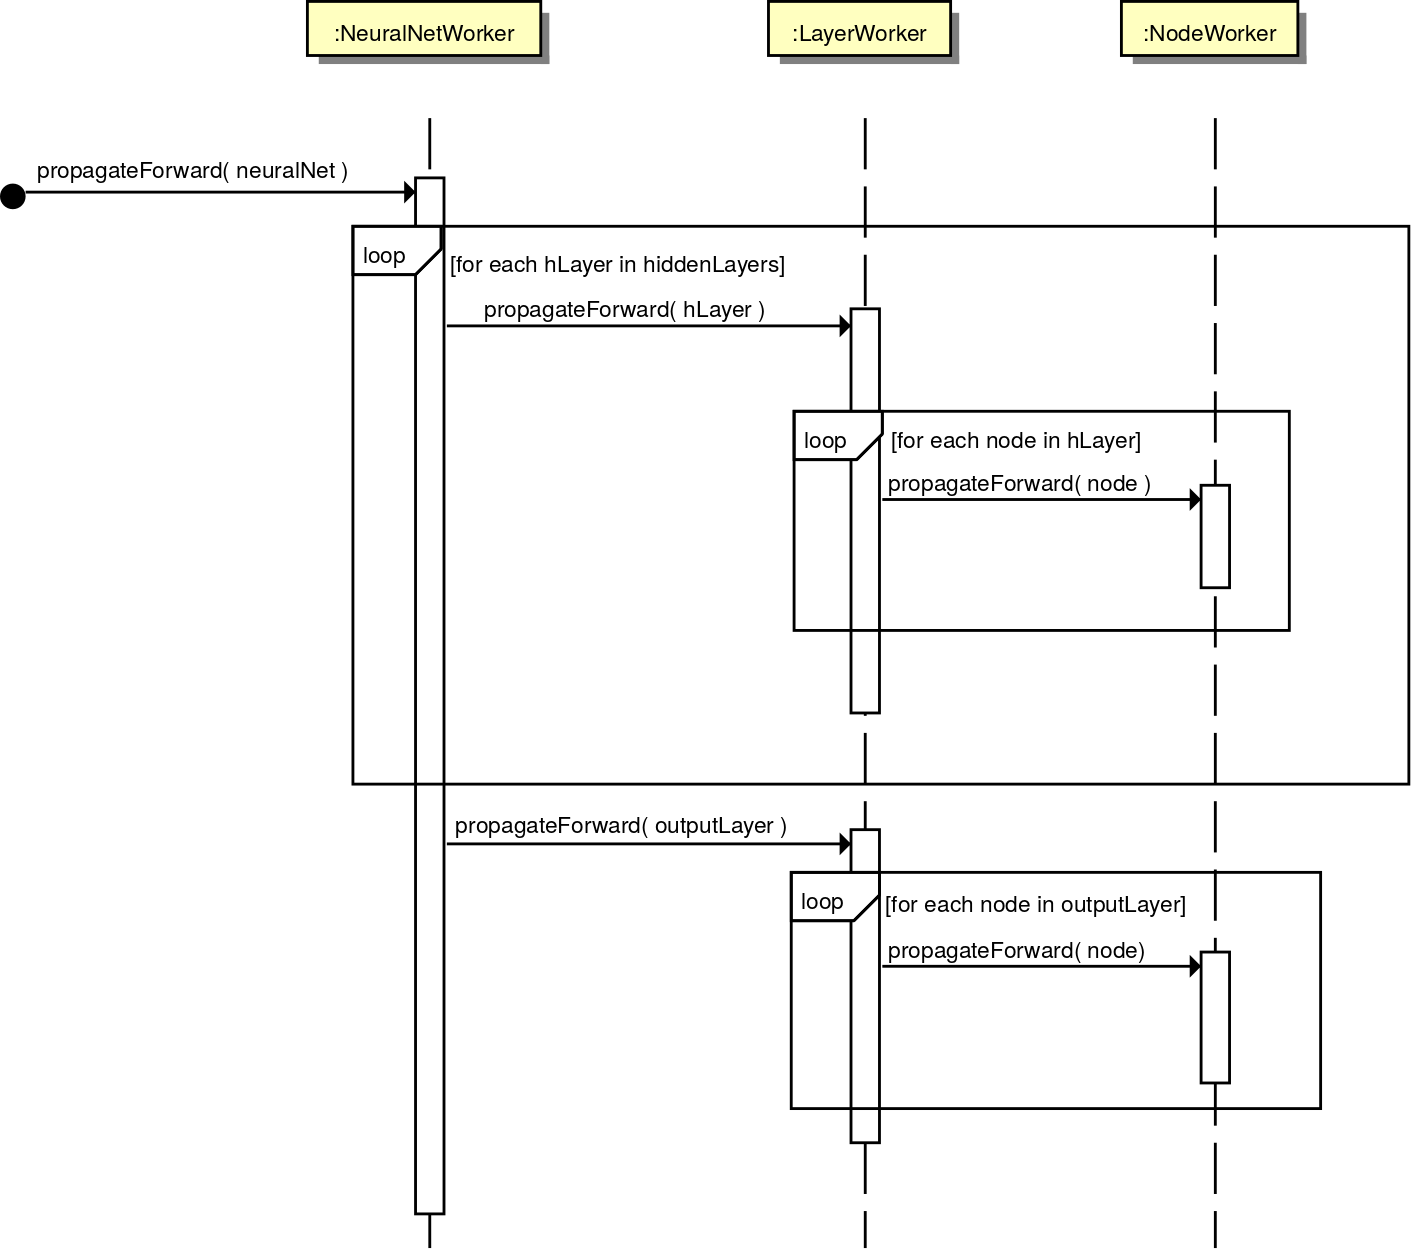
\includegraphics[width=13cm]{Abbildungen/UML/uml_ronny/forwardPropagationSD.png}
\end{center}
\end{figure}

\begin{figure}[H]
\begin{center}
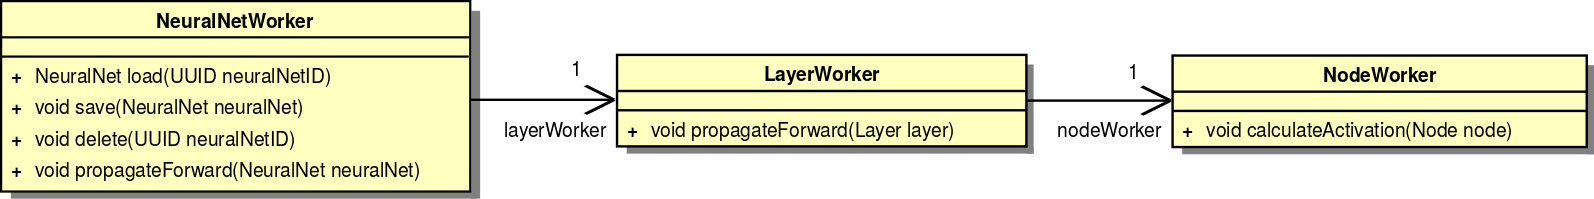
\includegraphics[width=\textwidth]{Abbildungen/UML/uml_ronny/workerKlassenDiagramm.png}
\end{center}
\end{figure}

\subsection{Administrationssicht}

\textbf{/F201/} Das Training eines Neuronalen Netzes erfolgt mit Hilfe des Gradienten-Abstieg-Algorithmus. Durch den Vergleich von tatsächlicher Netzwerkausgabe zur erwarteten Ausgabe werden dabei beginnend beim Ausgabelayer sukzessive Anpassungen an den Netzwerkknoten und Netzwerkaxon vorgenommen. Für jede Abstraktionstufe des Neuronalen Netzes wird dabei ein eigener Trainer angelegt, der für die Rückwärtspropagierung des Ausgabefehlers zuständig ist.\\[-0.5cm]
\begin{figure}[H]
\begin{center}
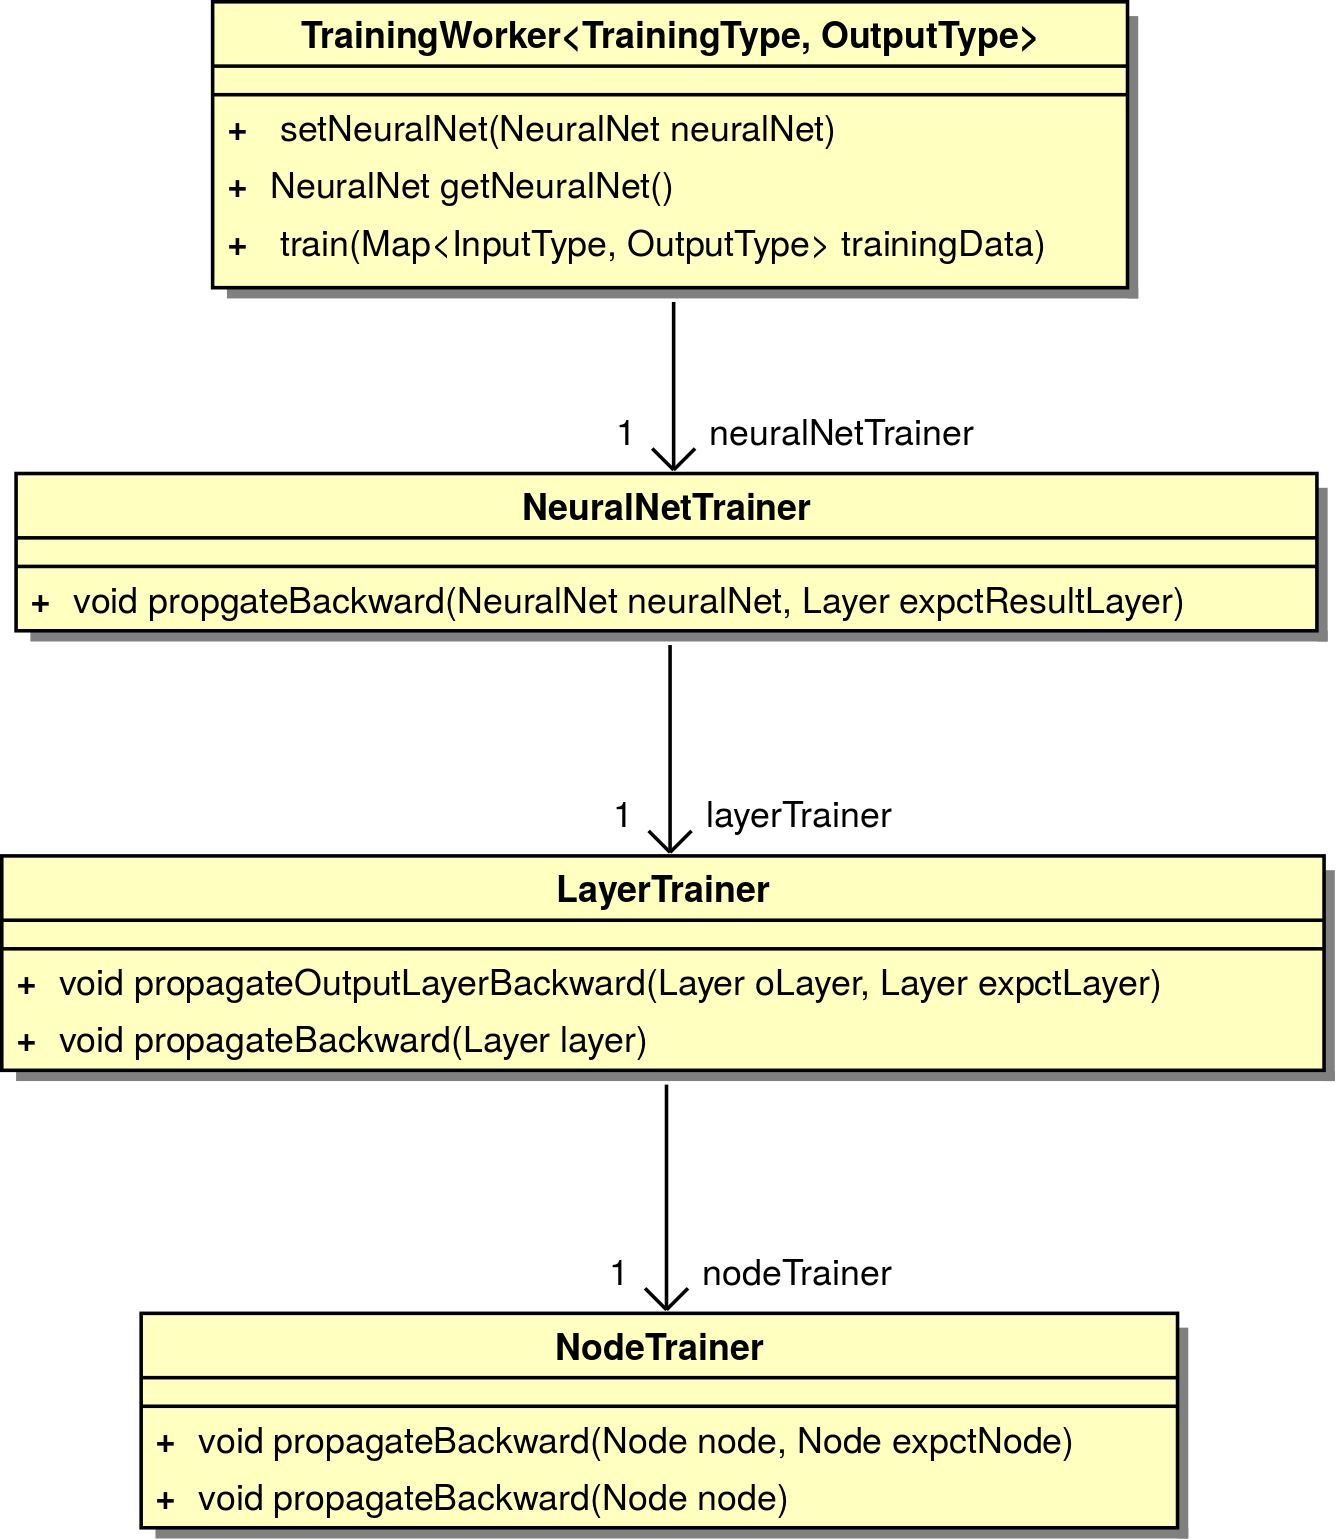
\includegraphics[width=10cm]{Abbildungen/UML/jan/trainerCD.png}
\caption{Klassendiagramm der Trainingsworker für das Neuronale Netz, Layer und Nodes.}
\label{fig_cdTraining}
\end{center}
\end{figure}
Der Ablauf eines Trainingdurchlaufs stellt sich als Sequenzdiagramm wie folgt dar:
\begin{figure}[H]
\begin{center}
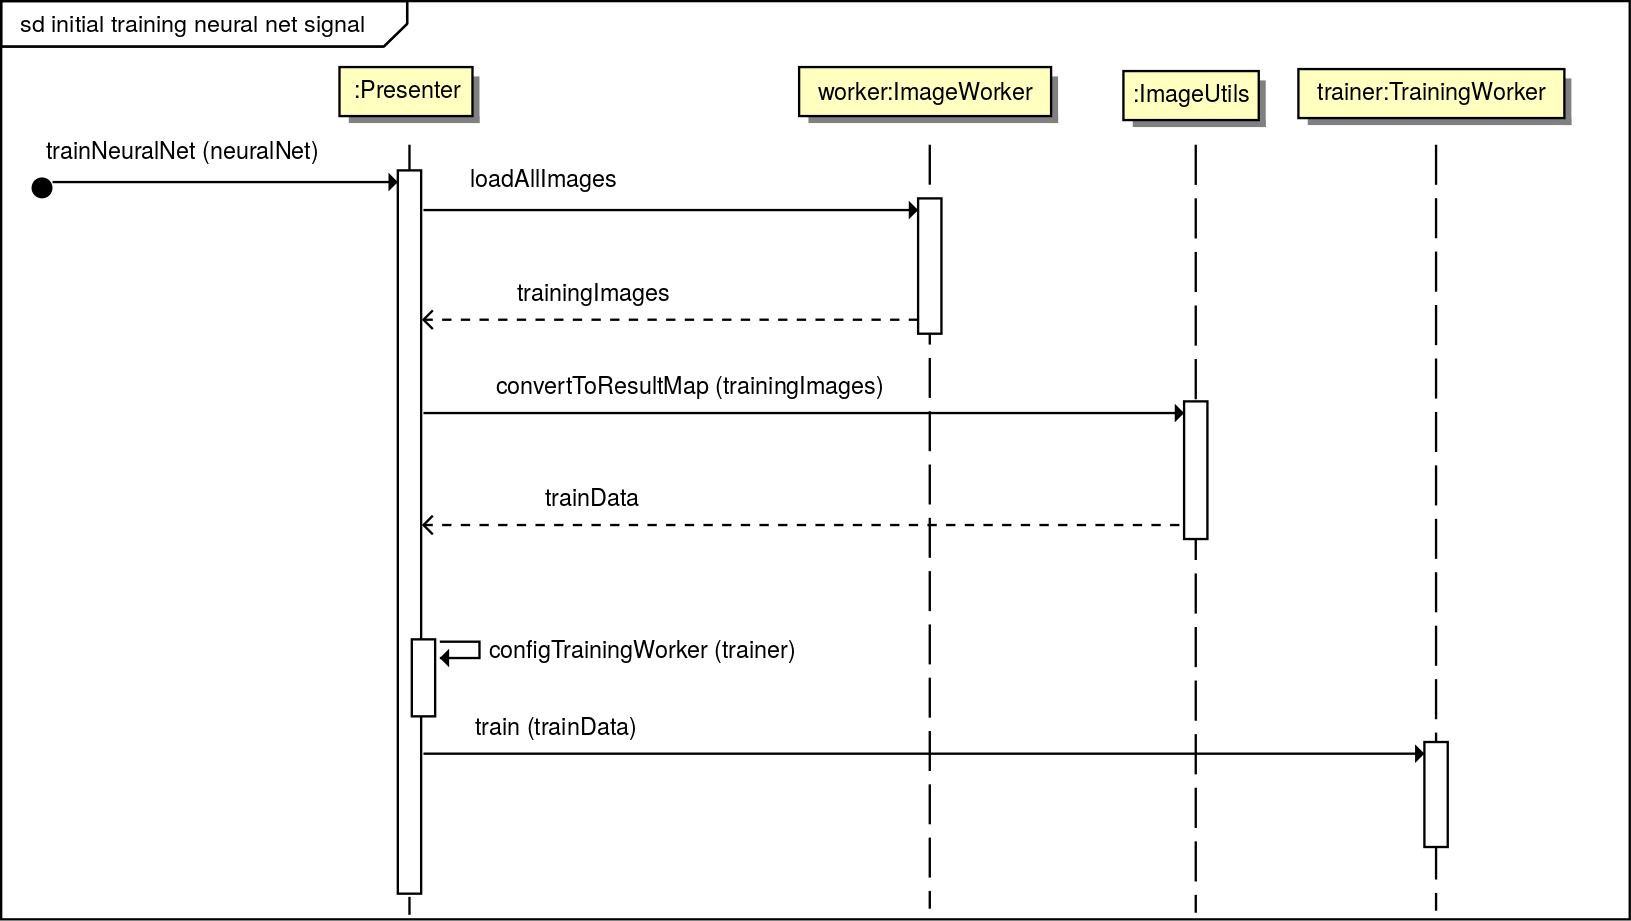
\includegraphics[width=14.2cm]{Abbildungen/UML/jan/trainNeuralNet.png}
\caption{Sequenzdiagramm zum Trainingsprozess beginnend am Presenter.}
\label{fig_sdTraining}
\end{center}
\end{figure}
\begin{figure}[H]
\begin{center}
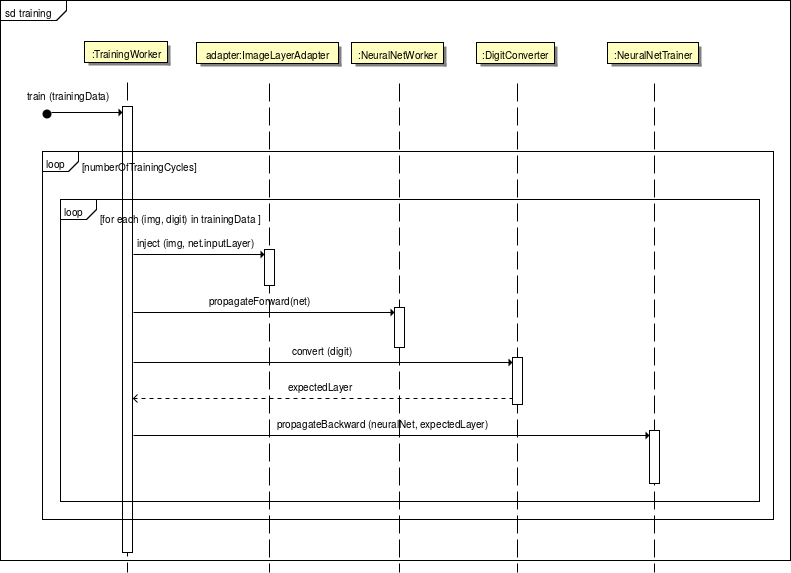
\includegraphics[width=14.2cm]{Abbildungen/UML/jan/trainDetailed1.png}
\caption{Sequenzdiagramm für Trainingsprozess im Trainingsworker.}
\label{fig_sdTraining}
\end{center}
\end{figure}
\vspace{-0.5cm}
\begin{figure}[H]
\begin{center}
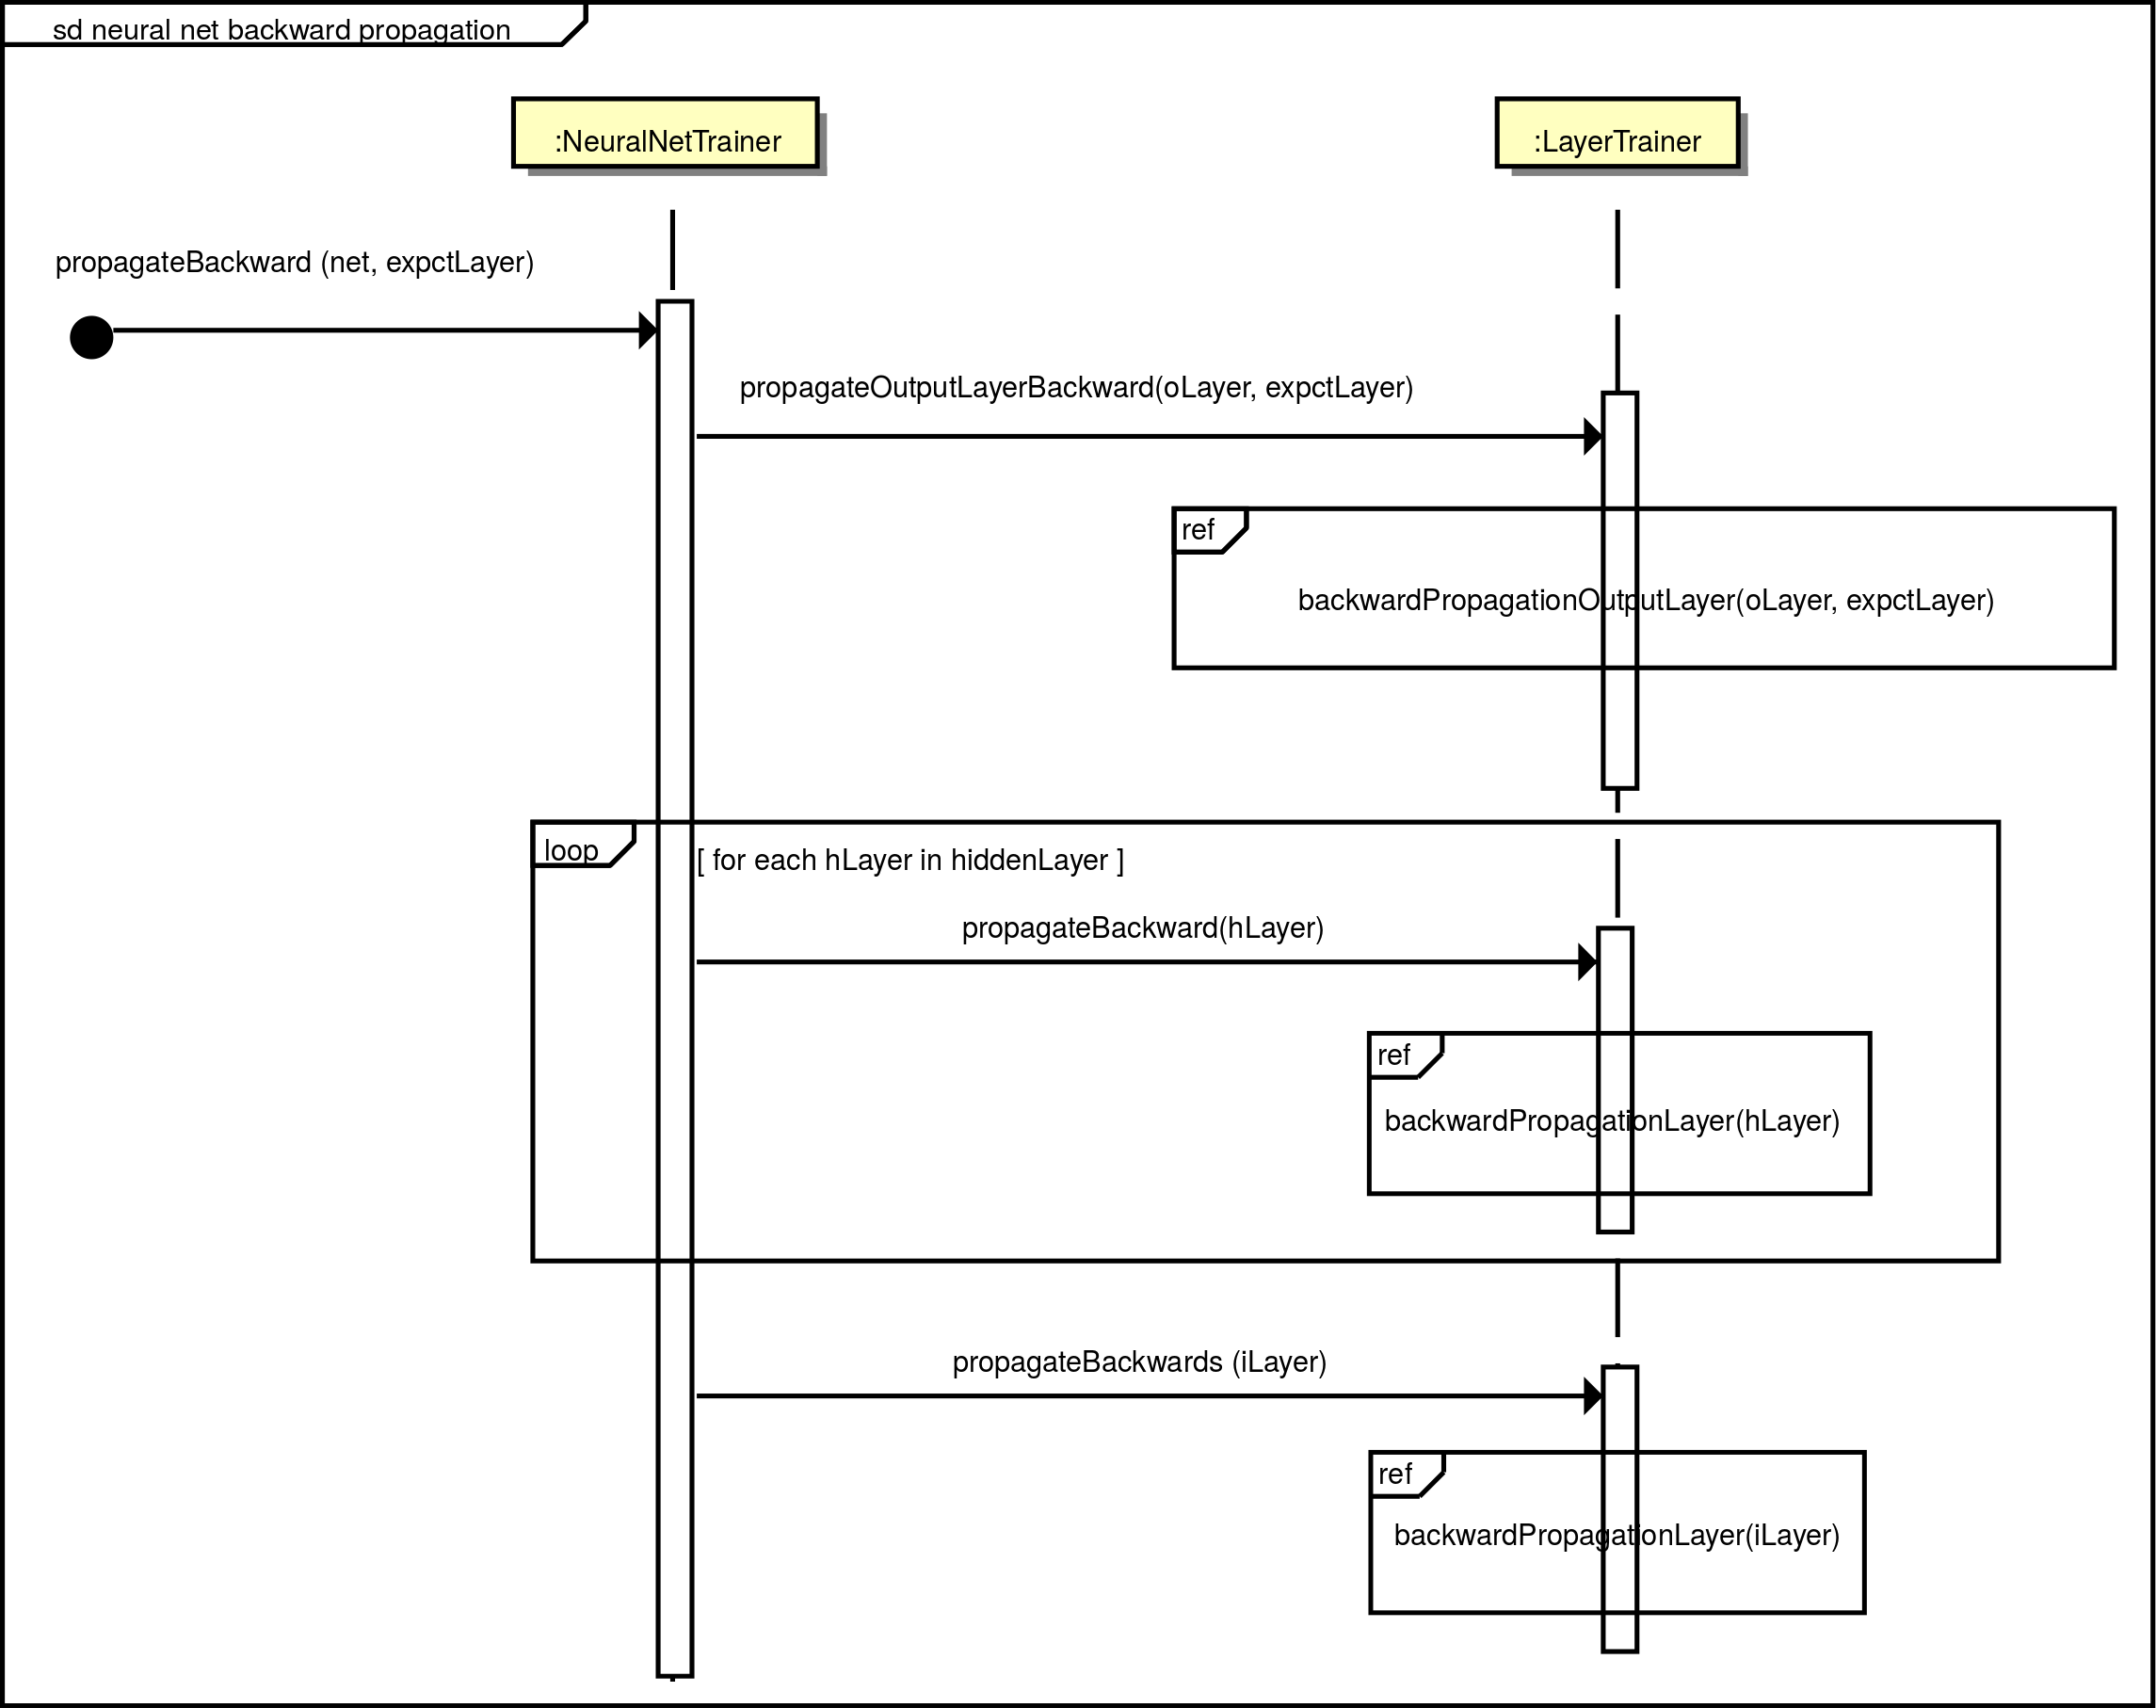
\includegraphics[width=15cm]{Abbildungen/UML/jan/gradientdescent1.png}
\caption{Sequenzdiagramm zur Backpropagation beginnend beim Neuronalen Netz.}
\label{fig_sdBackpropagation}
\end{center}
\end{figure}

\textbf{/F301/} 
\begin{figure}[H]
\begin{center}
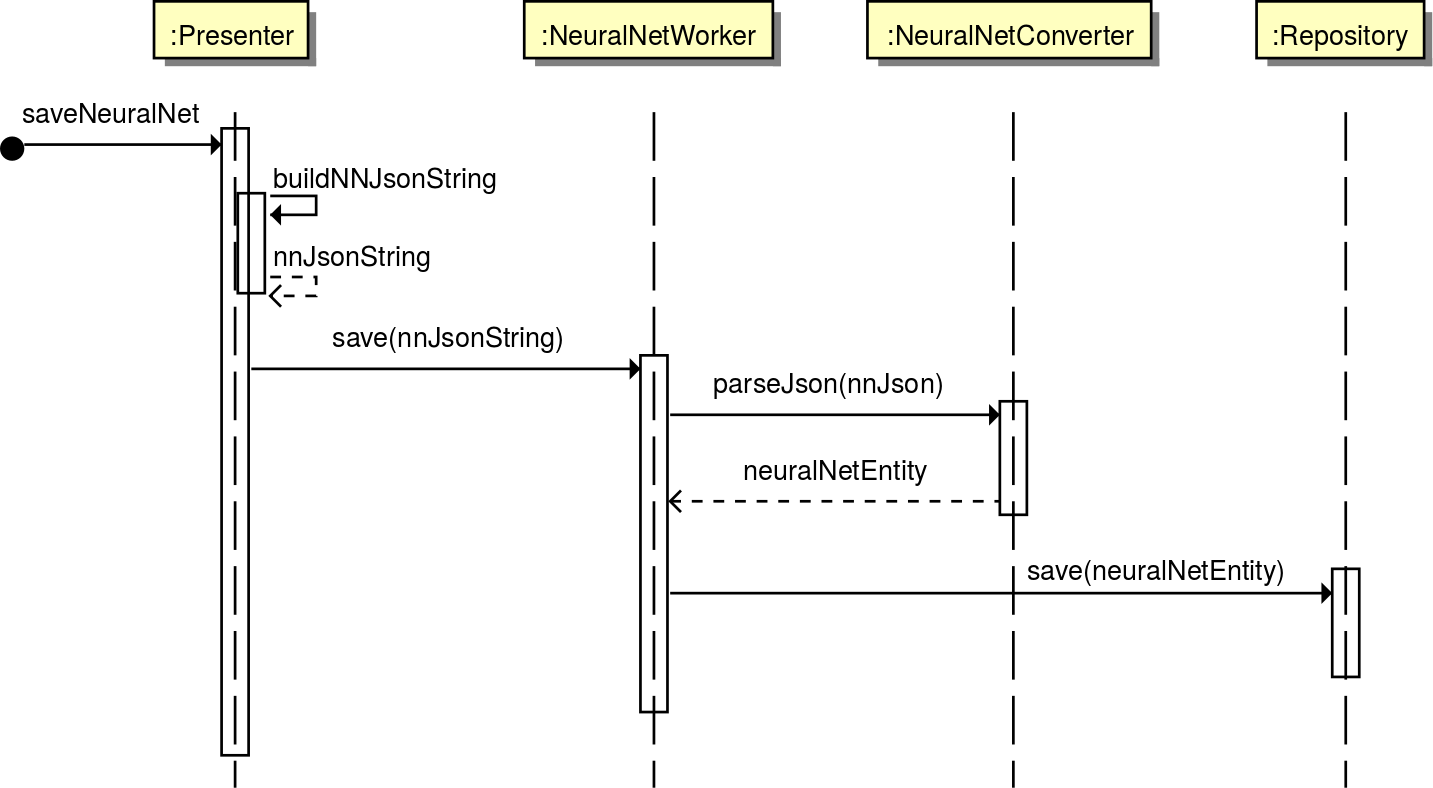
\includegraphics[width=15cm]{Abbildungen/UML/jan/convertJsonNNSD.png}
\caption{Sequenzdiagramm zur Konvertierung eines Json-Strings in ein Neuronalen Netz.}
\label{fig_sdBackpropagation}
\end{center}
\end{figure}
